%READ ONLY LÄNK
%https://www.overleaf.com/read/hfrdcszwfcsy
% ---------------- %%% A4 konvertering %%% ----------------- %
% ---------------- %%%    AVANCERAT    %%% ----------------- %
\documentclass[12pt]{article}
\usepackage[portrait,a4paper,margin=0cm]{geometry}
\usepackage[utf8]{inputenc}
\usepackage[T1]{fontenc}
\usepackage[swedish]{babel}
\usepackage{pdfpages}
\usepackage{filecontents}
\begin{filecontents*}{config.tex}
% ---------------------------------------------------------- %


% ---------------- %%% FORMATERING %%% ----------------- %

\documentclass[12pt]{article}
%% Import %%
\usepackage[paperwidth=105mm,paperheight=297mm,margin=1cm]{geometry}
\usepackage[utf8]{inputenc}
\usepackage[T1]{fontenc}
\usepackage[swedish]{babel}
\usepackage{amsmath}
\usepackage{lmodern}
\usepackage{units}
\usepackage{icomma}
\usepackage{color}
\usepackage{graphicx}
\usepackage{bbm}
\usepackage{hyperref}
\pagenumbering{gobble}
\usepackage{multicol}
\usepackage{titlesec}
\usepackage{mathtools}
\newcommand{\orientation}{\landskap}
\usepackage{etoolbox}
%% --- %%

%% Section-format %%
\setlength{\columnsep}{1.5cm}
\titleformat
{\section} % command
[display] % shape
{\bfseries\Large\itshape} % format
{} % label
{0em} % sep
{\vspace{-0.5em}\hspace{-0.05em}} % before-code
[\vspace{0em}] % after-code
\titlespacing{\section}{0em}{0em}{0.2em}
\setlength{\parindent}{0cm}
%% --- %%

%% Titelformat %%
\newcommand{\titelsida}
{
\begin{center}
\IfFileExists{logo.png}{
\includegraphics[width=\logga]{logo.png}~\\[0.75em]}{\vspace*{0.1\paperheight}}
\expandafter\ifblank\expandafter{\titel}{}{ \Huge \titel \\[0.75em] }
\expandafter\ifblank\expandafter{\host}{}{\large Toastmasters: \host\\[0.5em]}%
\expandafter\ifblank\expandafter{\datum}{}{\large \datum\\\vspace{0.6em}}
\expandafter\ifblank\expandafter{\forratt}{}{\large Förrätt: \forratt\\\vspace{0.1em}}
\expandafter\ifblank\expandafter{\huvudratt}{}{\large Huvudrätt: \huvudratt\\\vspace{0.1em}}
\expandafter\ifblank\expandafter{\efterratt}{}{\large Efterrätt: \efterratt\\\vspace{0.1em}}
\end{center}
}
%% --- %%

%% Sång %%
\newcommand{\inputsong}[1]{\input{../texter/#1.tex}}
%% --- %%

% Environment for songs
\newenvironment{song}[2]{
\section{#1}
\label{#2}
}{}

% Environment for verses
\newenvironment{vers}{
\begin{flushleft}\filbreak
}{
\end{flushleft}{}
}

% Definiera melodirad
\newcommand{\mel}[1]{\begin{flushleft}\textit{\small{Mel: #1}}\end{flushleft}}
% Ta bort eventuella kommentarer i sånghäftet
\newcommand{\av}[1]{}
\newcommand{\kom}[1]{}


% Repriser sheet music
\newcommand{\repopen}
{
	\raisebox{-.4ex}{\rule{.2ex}{2.5ex}\,\rule{.1ex}{2.5ex}}
	\hspace{-0.4ex}\raisebox{.2ex}{:}
}
\newcommand{\repclose}
{
	\raisebox{.2ex}{:}\hspace{-0.4ex}
	\raisebox{-.4ex}{\rule{.1ex}{2.5ex}\,\rule{.2ex}{2.5ex}}
}

% Definiera om sidbrytningar från sjungboken till ingenting - ändra inte
\newcommand{\newp}{}
%% --- %%


% -------------- %%% EGNA INSTÄLLNINGAR %%% -------------- %

%% Om något värde ej önskas, lämna måsvingarna tomma %%

%% Storlek på logga %%
%% Om ingen logga önskas, radera logo.png %%
\newcommand{\logga}
{0.8\textwidth}
%% --- %%

%% Titel %%
\newcommand{\titel}
{Titel}
%% --- %%

%% Värdar/Toastmasters %%
\newcommand{\host}
{Värd}
%% --- %%

%% Meny %%
\newcommand{\forratt}
{Förrätt}
\newcommand{\huvudratt}
{Huvudrätt}
\newcommand{\efterratt}
{Efterrätt}
%% --- %%

%% Datum %%
\newcommand{\datum}
{den \today}
%% --- %%

%% Melodirad %%
% Exkludera melodirad (avkommentera om du vill att melodiraden ska gömmas)
%\renewcommand{\mel}[1]{} % Ingen melodirad
%% --- %%

%% Repristecken %%
% Avkommentera båda om du vill byta ut repristecknet mot textekvivalent
%\renewcommand{\repopen}{//:}
%\renewcommand{\repclose}{://}
%% --- %%

% ------------------- %%% DOKUMENT %%% ------------------- %

\begin{document}
\titelsida
\inputsong{livet}
\inputsong{porthos}
\inputsong{vikingen}
\inputsong{fetafransyskor}
\inputsong{bordeaux}
\inputsong{strejkpapripps}
\inputsong{gamlakall}
\newpage
\inputsong{sistapunschvisan}
\end{document}

% -------------------------------------------------------- %


























% ---------------- %%%     RÖR EJ      %%% ----------------- %
\end{filecontents*}

\makeatletter
\def\app@exe{\immediate\write18} % Definiera körbara Linux-kommandon
\def\createBooklet{%
    \app@exe{pdflatex config.tex}% Kompilera config.tex som har skapats genom filecontents-paketet

    % Räkna antalet sidor
    \pdfximage{config.pdf}
    
    % Väljer automatiskt rätt layout för antalet sidor
    
    % 1-2
    \ifnum\the\pdflastximagepages=1
        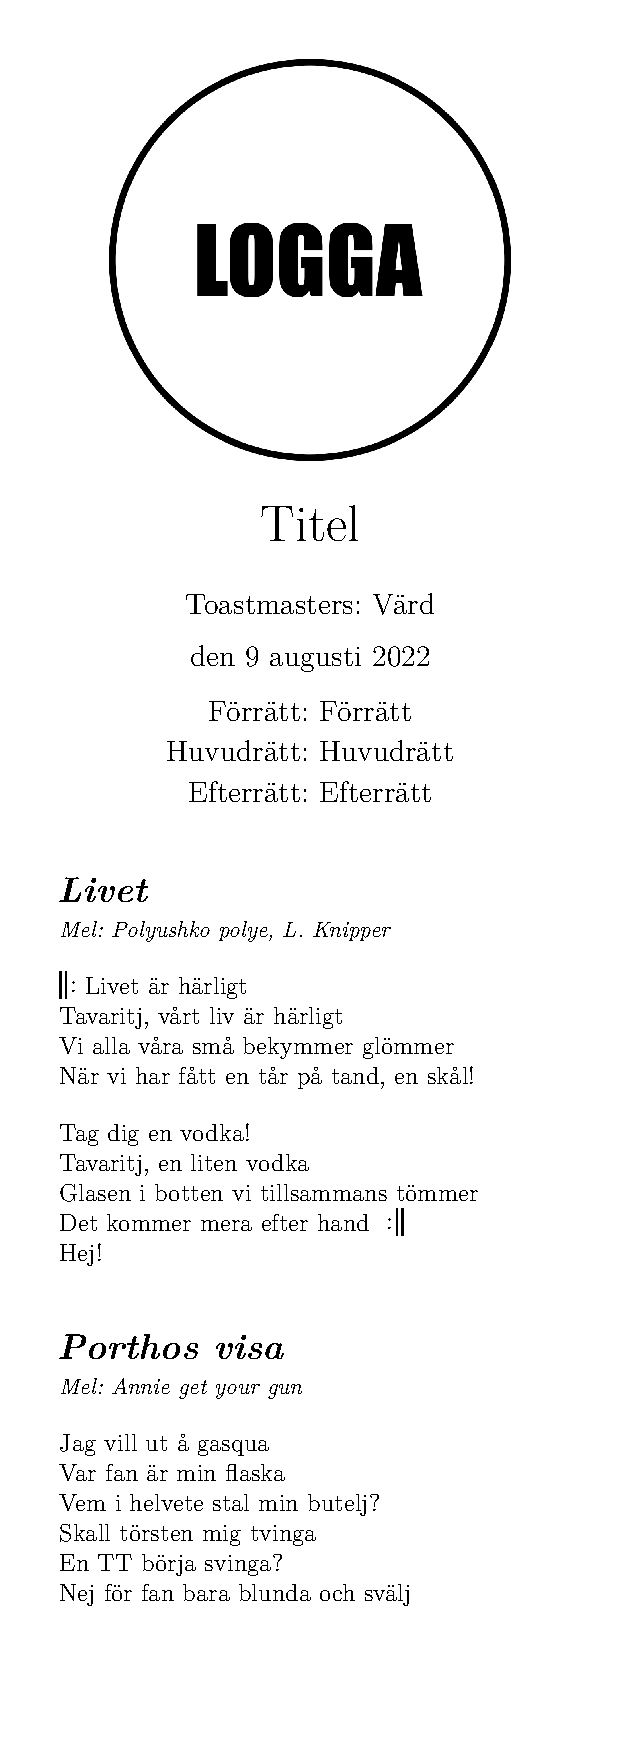
\includepdf[pages=-,nup=2x1]{config.pdf}
    \fi
    \ifnum\the\pdflastximagepages=2
        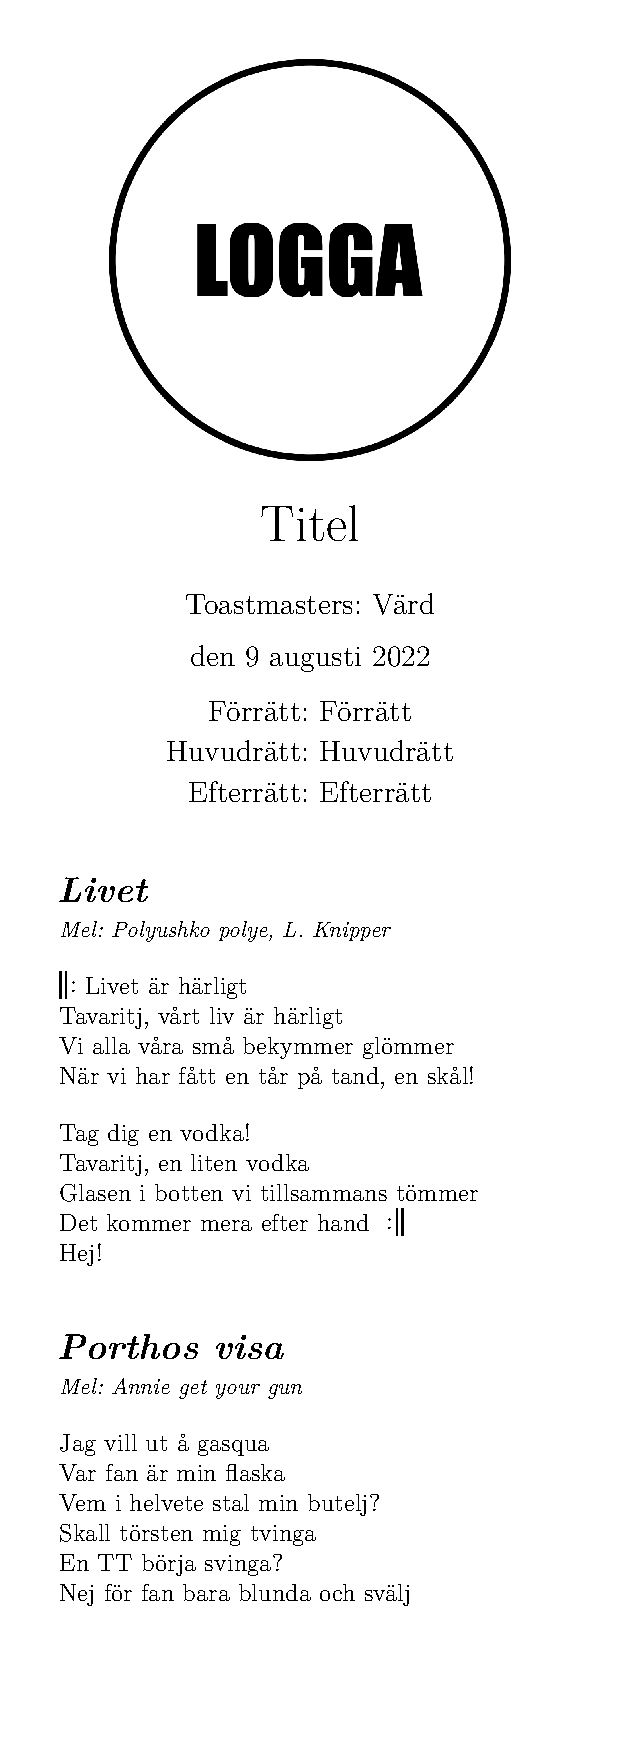
\includepdf[pages=-,nup=2x1]{config.pdf}
    \fi
    
    % 3-4
    \ifnum\the\pdflastximagepages=3
        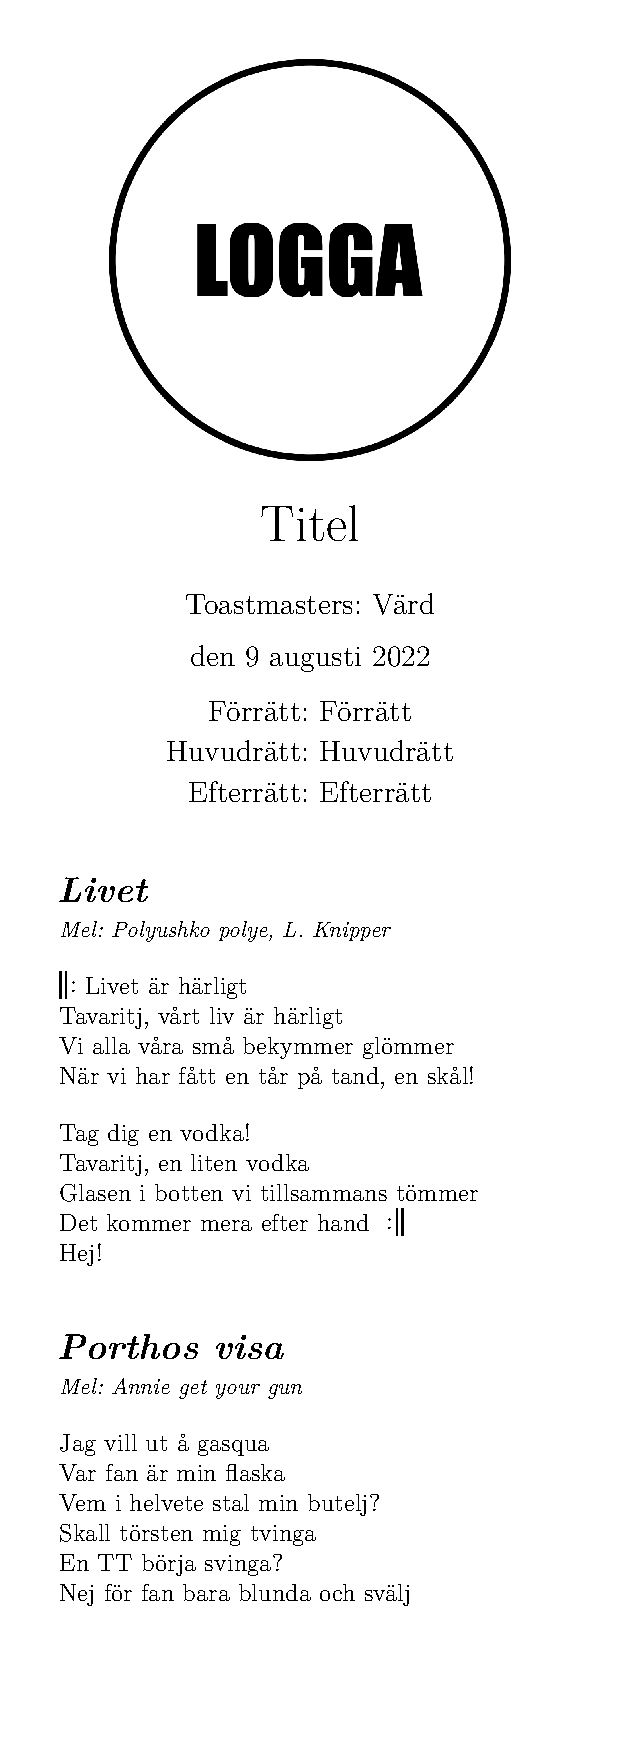
\includepdf[pages={{},1,2,3},nup=2x1]{config.pdf}
    \fi
    \ifnum\the\pdflastximagepages=4
        \includepdf[pages={4,1,2,3},nup=2x1]{config.pdf}
    \fi
    
    % 5-8
    \ifnum\the\pdflastximagepages=5
        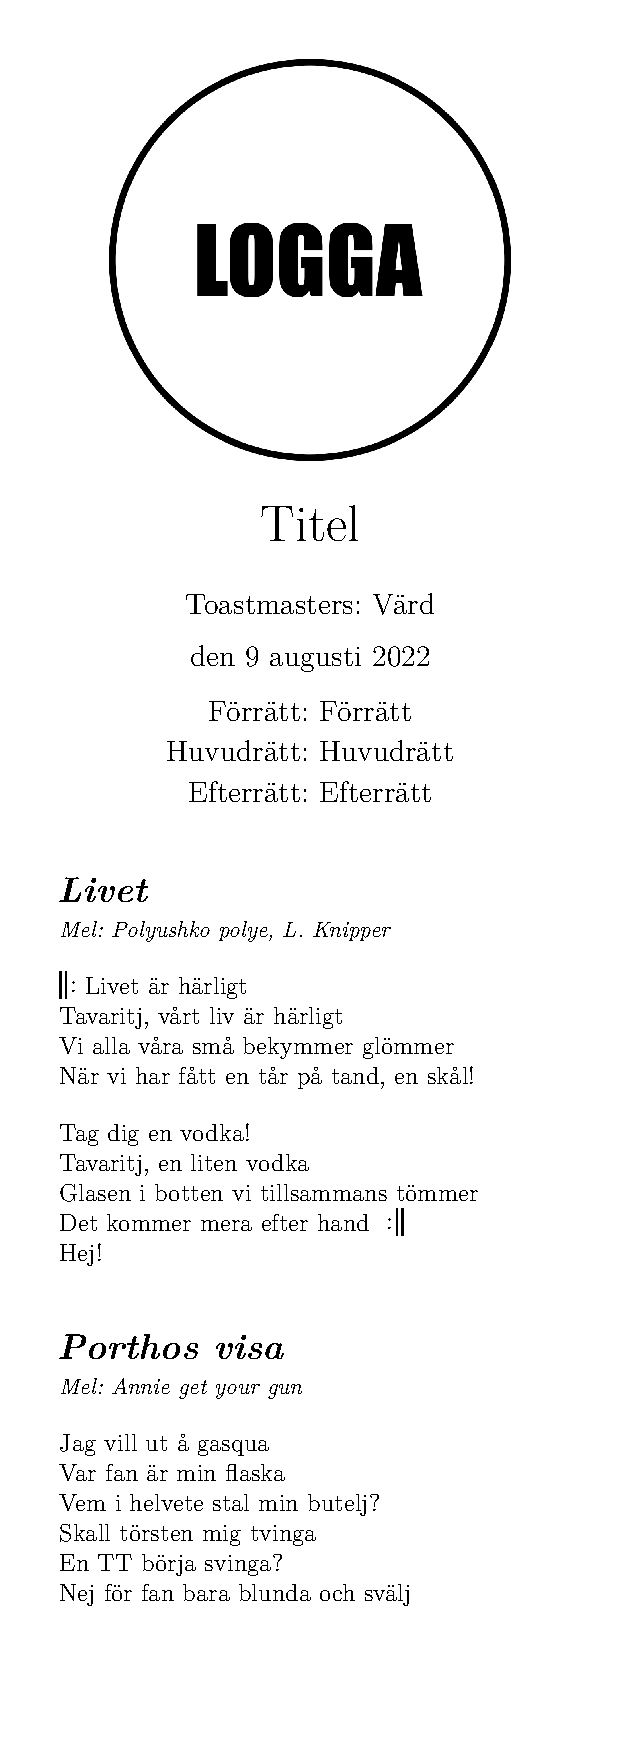
\includepdf[pages={{},1,2,{},{},3,4,5},nup=2x1]{config.pdf}
    \fi
    \ifnum\the\pdflastximagepages=6
        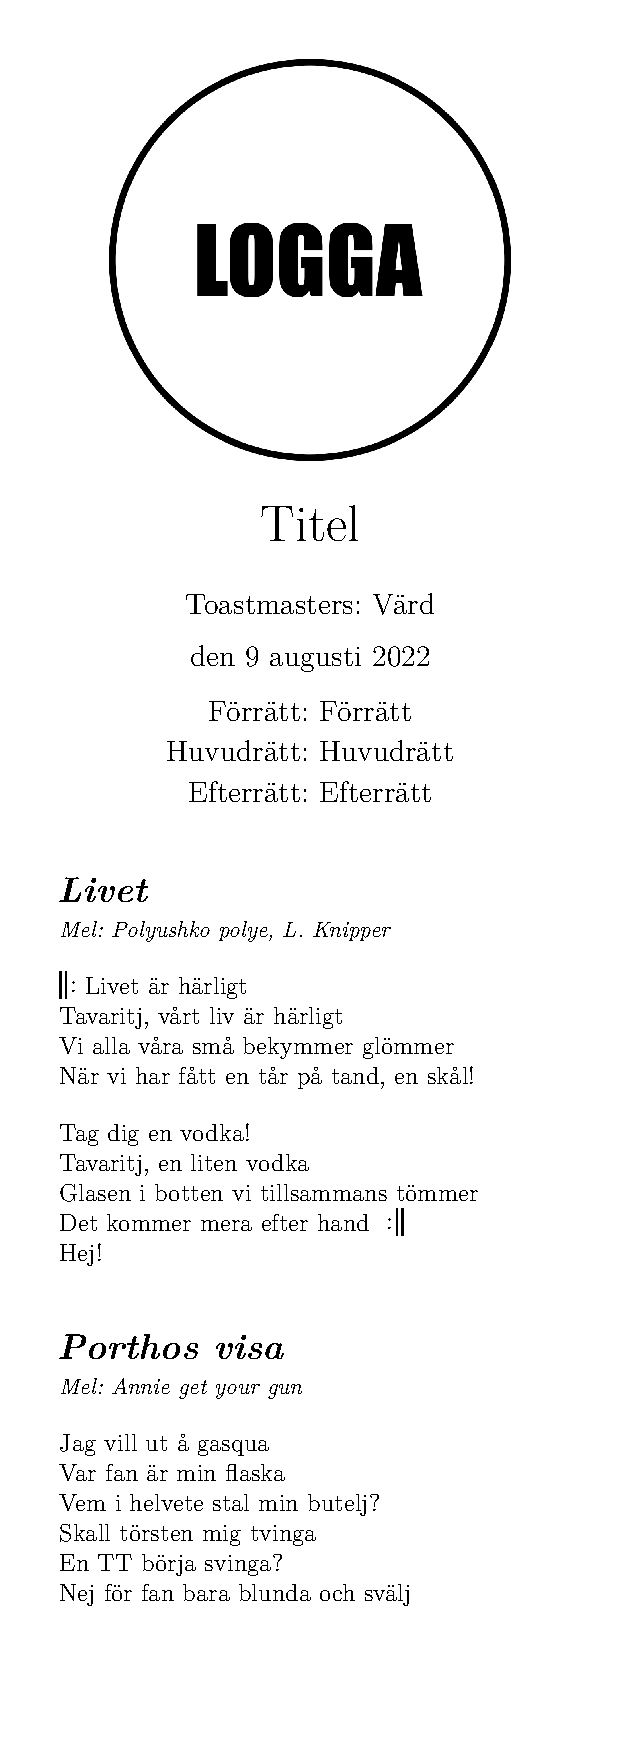
\includepdf[pages={{},1,2,{},6,3,4,5},nup=2x1]{config.pdf}
    \fi
    \ifnum\the\pdflastximagepages=7
        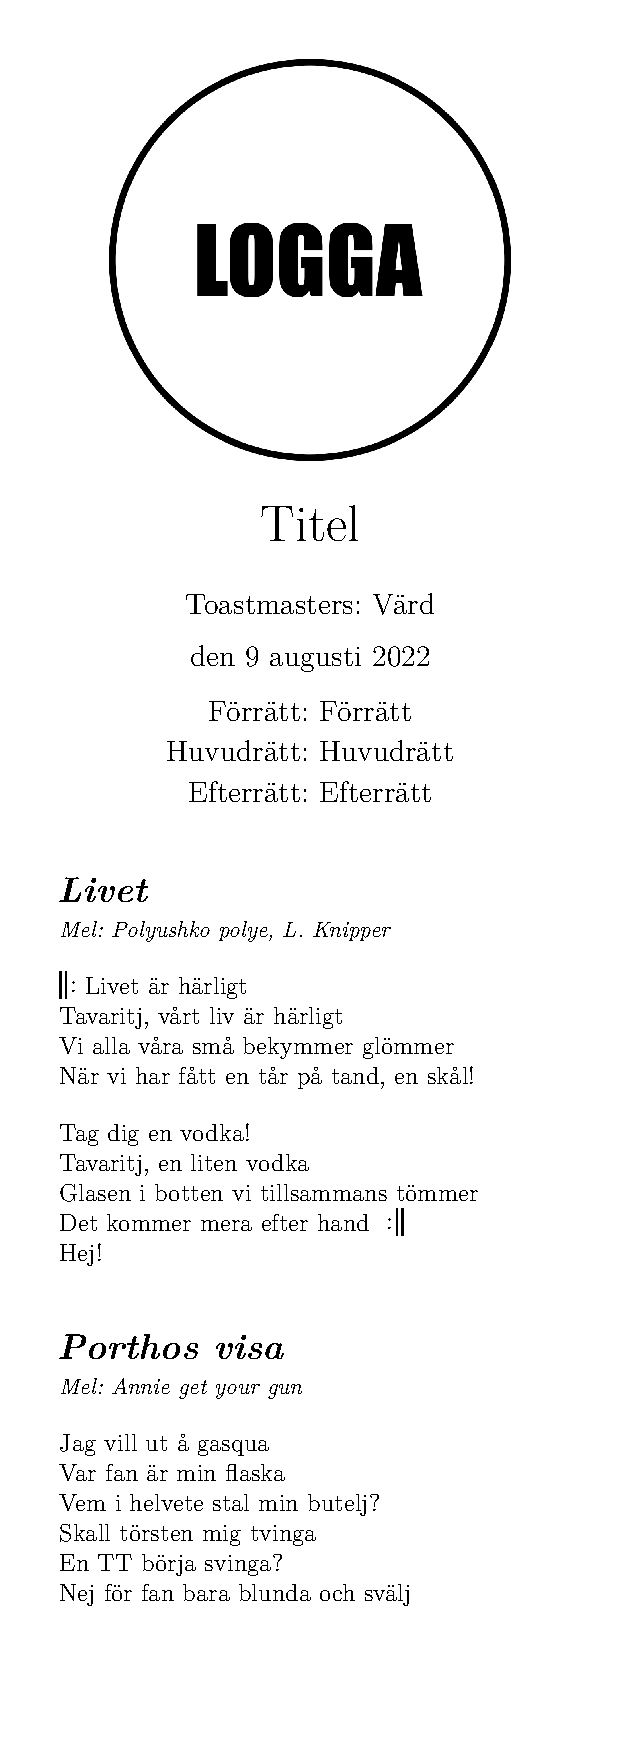
\includepdf[pages={{},1,2,7,6,3,4,5},nup=2x1]{config.pdf}
    \fi
    \ifnum\the\pdflastximagepages=8
        \includepdf[pages={8,1,2,7,6,3,4,5},nup=2x1]{config.pdf}
    \fi
    
    % 9-12
    \ifnum\the\pdflastximagepages=9
        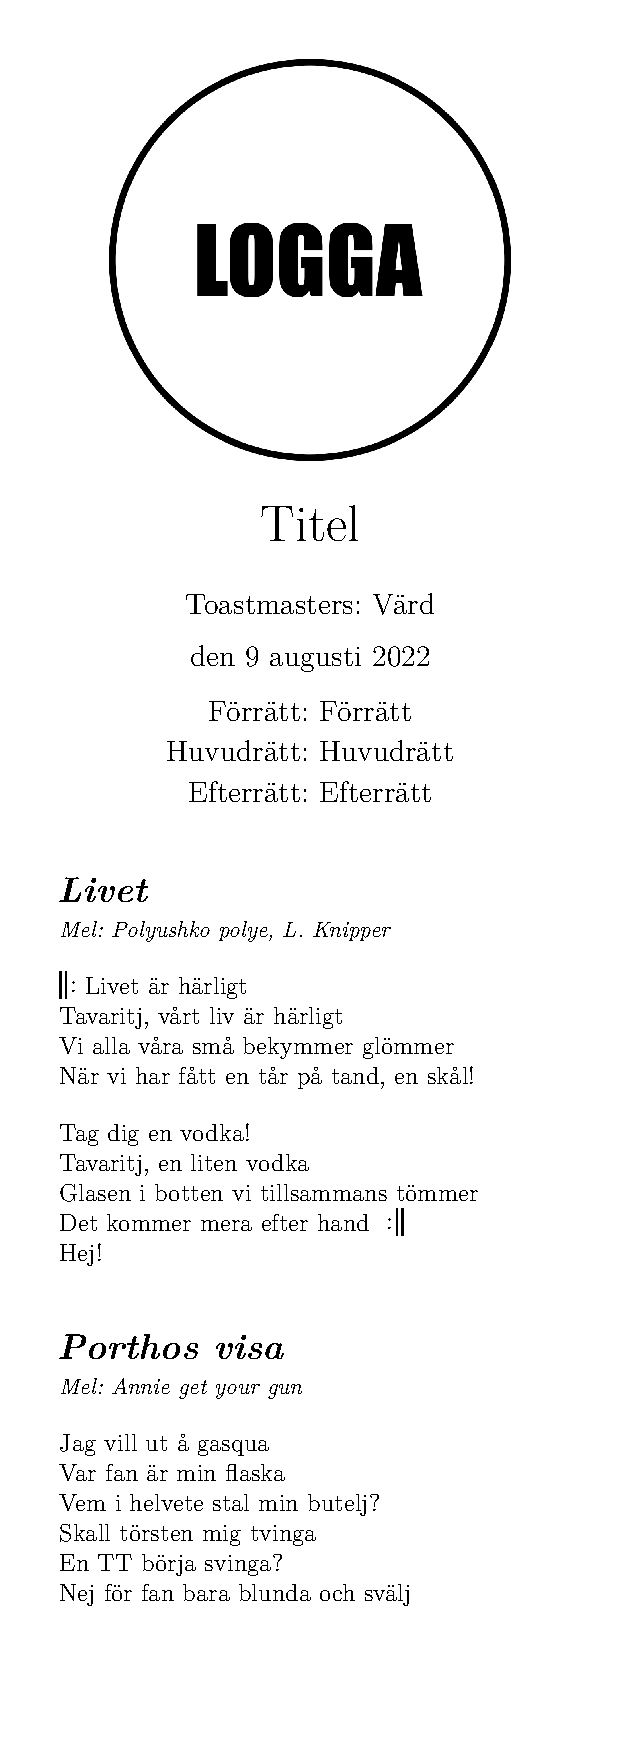
\includepdf[pages={{},1,2,{},{},3,4,9,8,5,6,7},nup=2x1]{config.pdf}
    \fi
    \ifnum\the\pdflastximagepages=10
        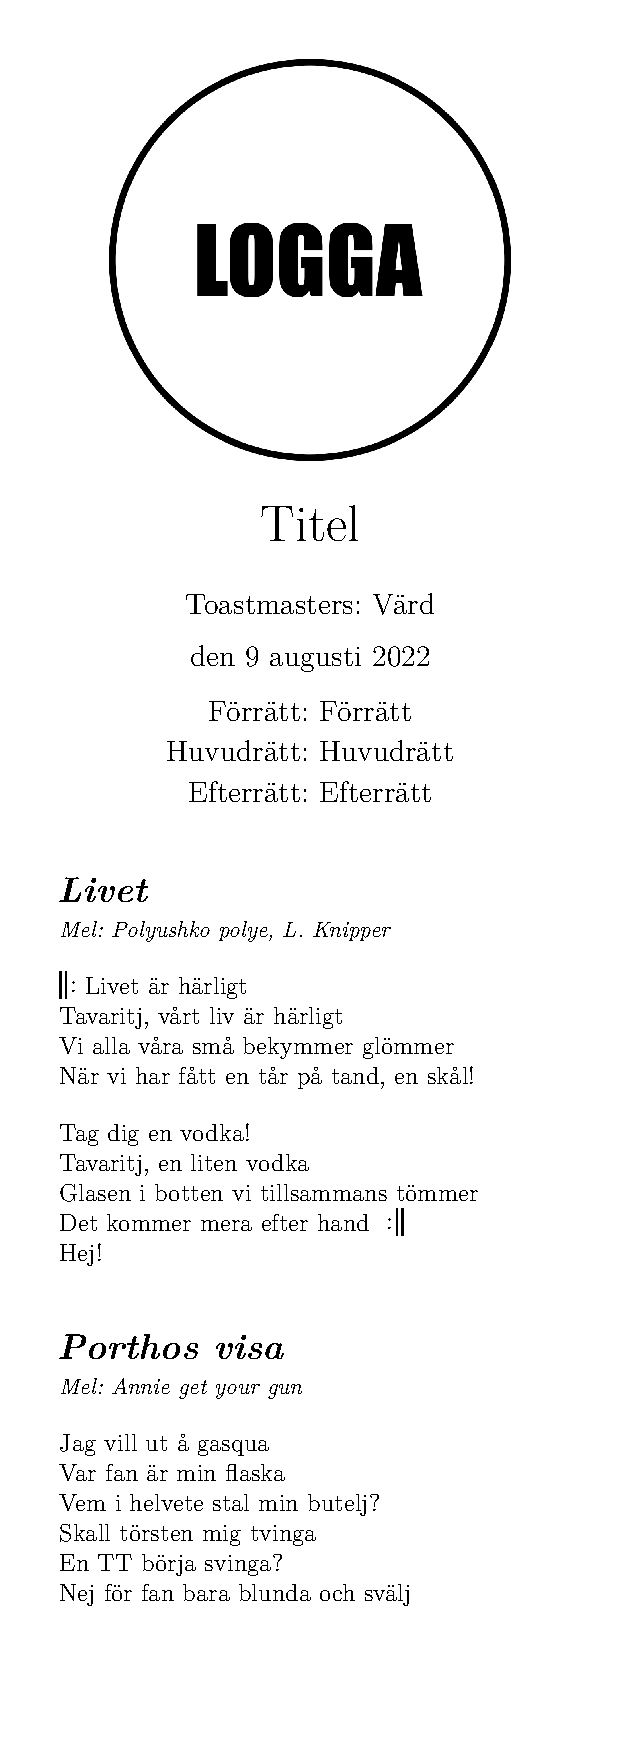
\includepdf[pages={{},1,2,{},10,3,4,9,8,5,6,7},nup=2x1]{config.pdf}
    \fi
    \ifnum\the\pdflastximagepages=11
        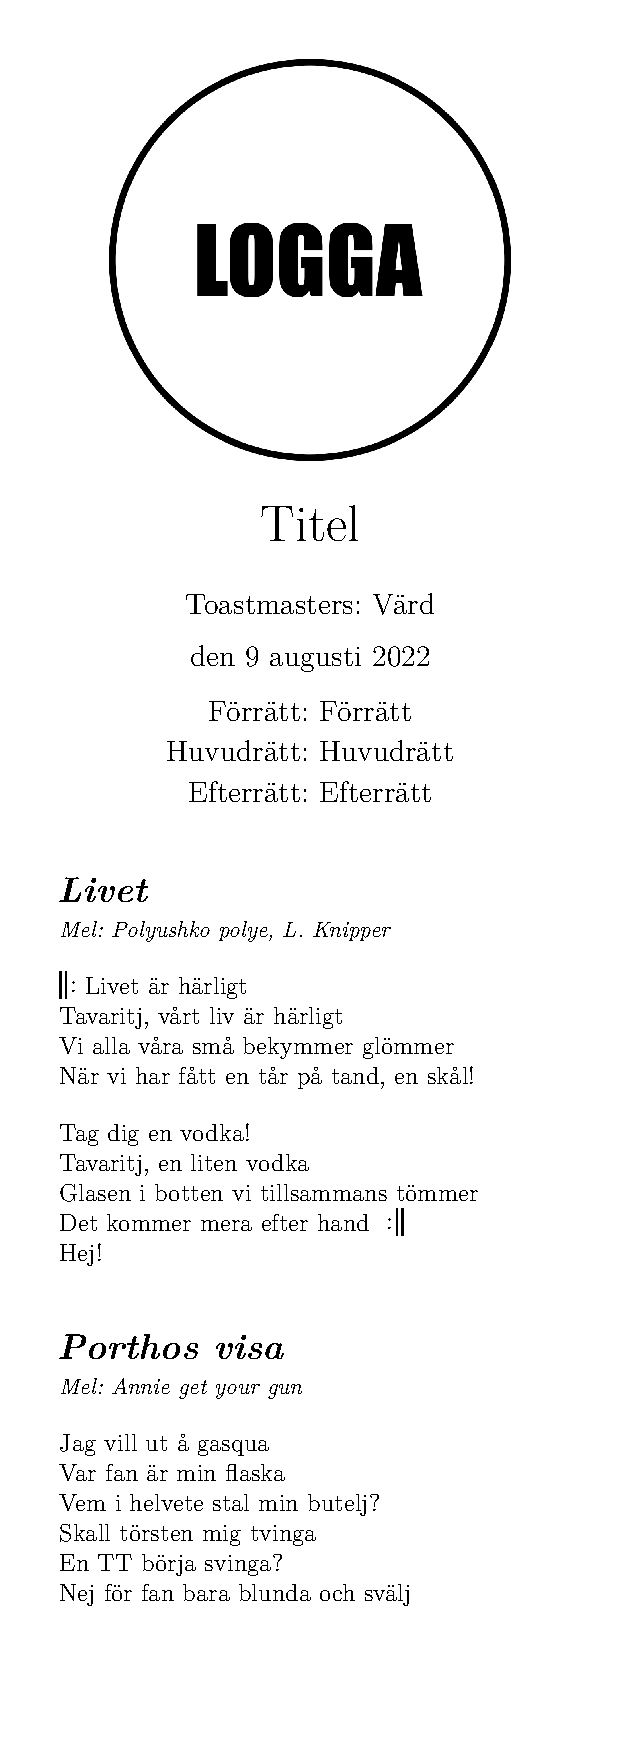
\includepdf[pages={{},1,2,11,10,3,4,9,8,5,6,7},nup=2x1]{config.pdf}
    \fi
    \ifnum\the\pdflastximagepages=12
        \includepdf[pages={12,1,2,11,10,3,4,9,8,5,6,7},nup=2x1]{config.pdf}
    \fi
    
    % 13-16
    \ifnum\the\pdflastximagepages=13
        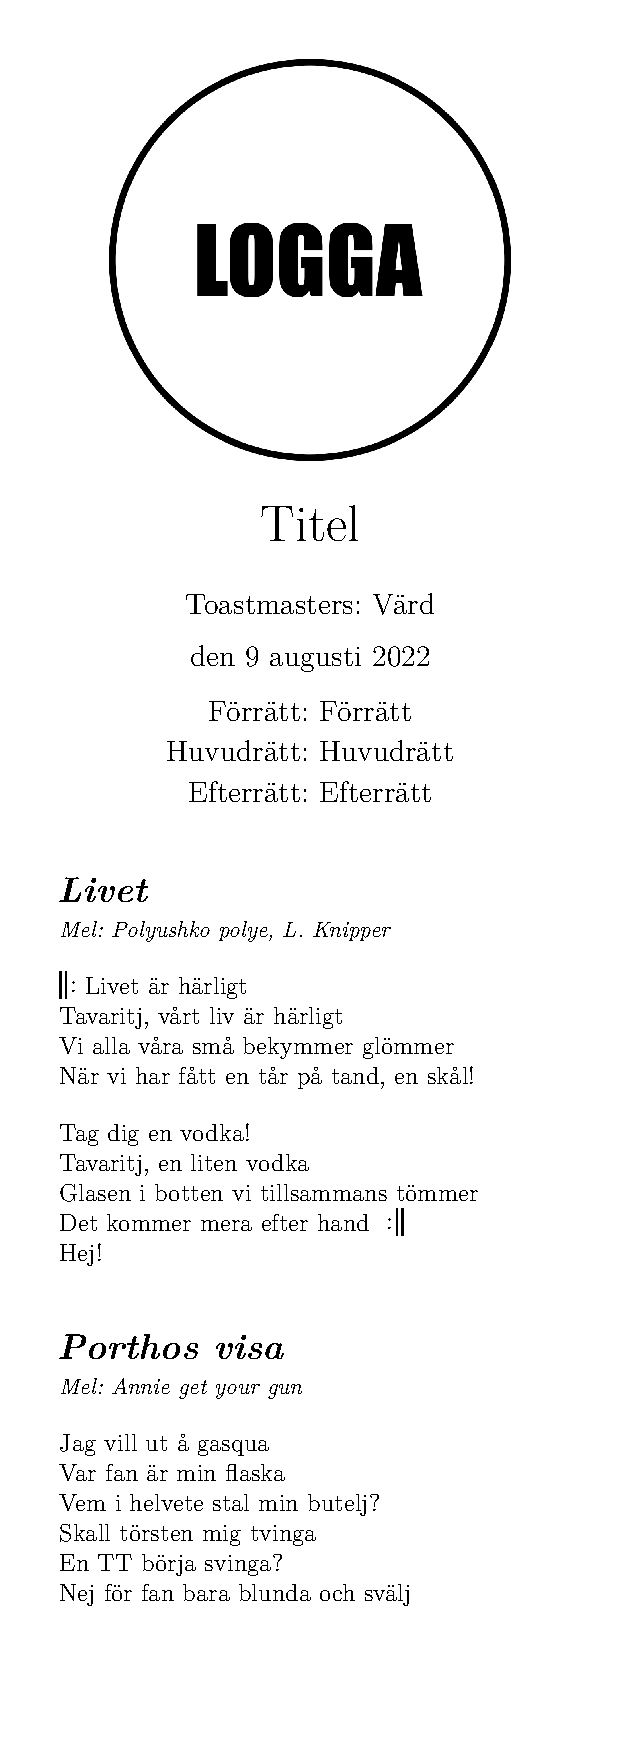
\includepdf[pages={{},1,2,{},{},3,4,13,12,5,6,11,10,7,8,9},nup=2x1]{config.pdf}
    \fi
    \ifnum\the\pdflastximagepages=14
        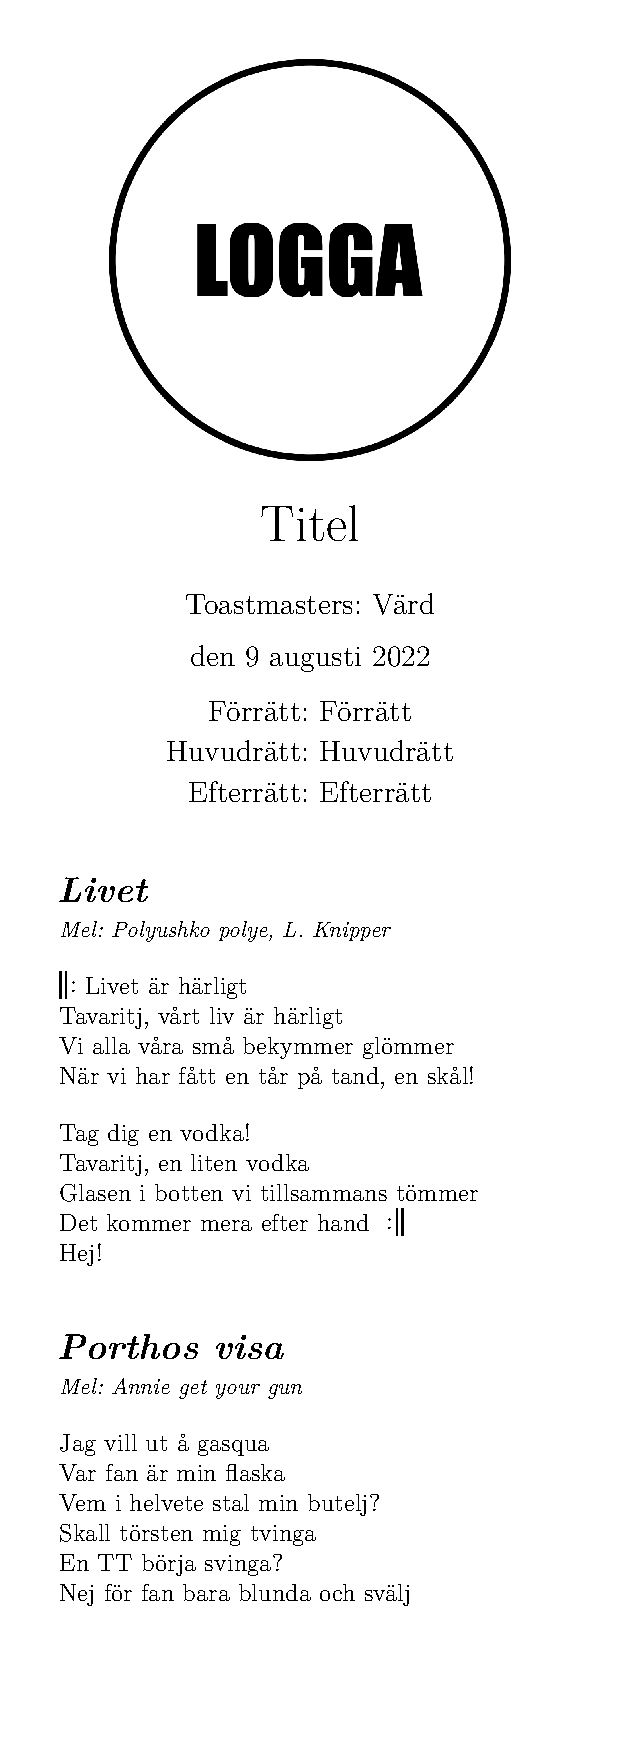
\includepdf[pages={{},1,2,{},14,3,4,13,12,5,6,11,10,7,8,9},nup=2x1]{config.pdf}
    \fi
    \ifnum\the\pdflastximagepages=15
        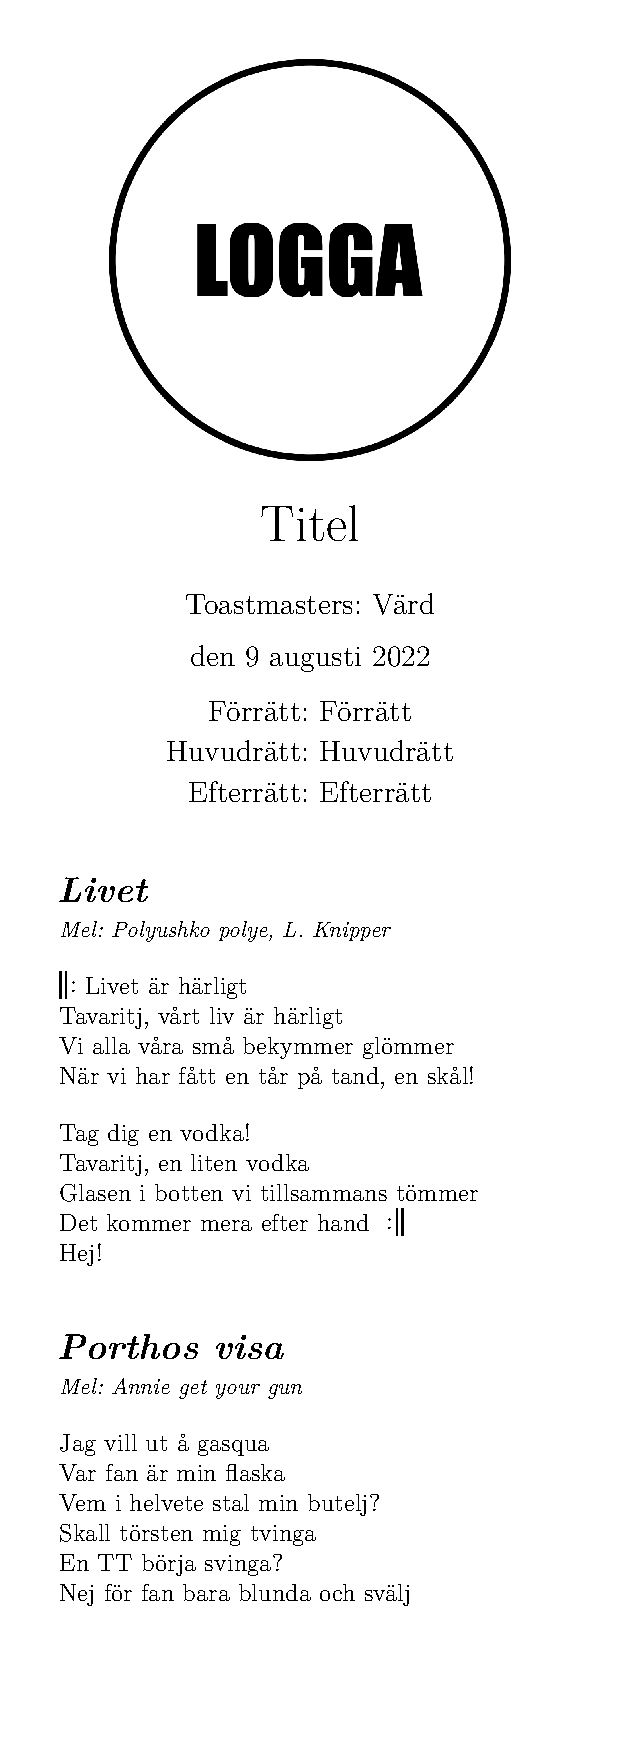
\includepdf[pages={{},1,2,15,14,3,4,13,12,5,6,11,10,7,8,9},nup=2x1]{config.pdf}
    \fi
    \ifnum\the\pdflastximagepages=16
        \includepdf[pages={16,1,2,15,14,3,4,13,12,5,6,11,10,7,8,9},nup=2x1]{config.pdf}
    \fi
    
}
\makeatother

\begin{document}
\createBooklet
\end{document}
